\section{Результаты}

\subsection{Audio quality}

We conduct the MOS (mean opinion score) evaluation for generated speech using Amazon Mechanical Turk. We compared four types of samples: 1) ground truth speech, 2) ground truth mel-spectrogram converted to speech with WaveGlow, 3) Tacotron 2 + WaveGlow, and 4) TalkNet + WaveGlow. We used NVIDIA's implementation for Tacotron 2 and WaveGlow. We tested $100$ audio samples with $10$ people per sample. The scores ranged from $1.0$ to $5.0$ with a step of $0.5$. TalkNet speech quality comes quite close to Tacotron 2 (see Table~\ref{tab:mos}). 

\begin{table}[!ht]
\centering
\scalebox{1.0}{
\begin{tabular}{l c} 
\toprule
\textbf{Model} &
\textbf{MOS} \\
\midrule
Ground truth speech & $4.31 \pm 0.05$ \\
Ground truth mel + WaveGlow & $4.04 \pm 0.05$ \\
Tacotron 2 + WaveGlow & $3.85 \pm 0.06$ \\
% FastSpeech~\cite{Fastspeech2019} & $\star \pm \star$ \\
\midrule
TalkNet + WaveGlow & $3.74 \pm 0.07$ \\
\bottomrule
\end{tabular}
}
\caption{MOS scores with $95\%$ confidence interval}
\label{tab:mos}
\end{table}

TalkNet is very robust with respect to missing or repeated words compared to auto-regressive TTS models such as Tacotron 2 or Transformer TTS. We evaluated the robust\-ness of TalkNet on 50 hard sentences from FastSpeech paper~\cite{fastspeech} and found that TalkNet eliminates missed or repeated words.

\subsection{Inference latency}

In the inference mode, we first insert blank symbols into the tokenized input text between every two characters. The obtained sequence is passed through the grapheme duration predictor. The output of the grapheme duration predictor is then corrected for characters with $0$ duration. The corrected character sequence is expanded with each character repeated according to the predicted duration. The second network generates the mel-spectrogram from the expanded grapheme sequence.

We compare the TalkNet inference latency with Tacotron 2 and FastSpeech. We used an internal NVIDIA FastSpeech implementation since the original FastSpeech was not available at the moment of evaluation. To measure the latency, we generate mel-spectro\-grams with a batch size equal 1 for 2048  samples from LJSpeech dataset. The average mel-spectrogram length is $520$ frames. We benchmark the latency on one V100 GPU. TalkNet inference is significantly faster than Tacotron 2 and FastSpeech (see Table~\ref{tab:lats}). Since TalkNet  does not use an attention mechanism, the inference latency practically does not depend on the input length.

\begin{table}[!ht]
\centering
\scalebox{1.0}{
\begin{tabular}{l  l r} 
\toprule
\textbf{Model} & 
% \textbf{\thead{\# Batch\\size}} &
\textbf{\thead{Inference\\Latency, s}} &
\textbf{RTF} \\
\midrule
% Transformer TTS~\cite{TransformerTTS} & 1 & $6.735 \pm 3.969$ & $1.48 \pm 0.87$ \\
Tacotron 2~\cite{tacotron2}  &$0.817 \pm 1\cdot 10^{-2} $ & $7.56 \pm 0.01$ \\
FastSpeech~\cite{fastspeech}  & $0.029 \pm 2 \cdot {10}^{-4}$  & $221.01 \pm 1.75$ \\
\midrule
TalkNet  &  $0.019 \pm 1 \cdot {10}^{-5}$ & $328.65 \pm \ \ 4.76$ \\
%  & 4 &   $0.023 \pm 5 \cdot {10}^{-5}$ & $1048.80 \pm 21.75$ \\
%  & 8 &  $0.037 \pm 4 \cdot {10}^{-4}$ & $1340.09 \pm \ \ 8.90$ \\
\bottomrule
\end{tabular}
}
\caption{TalkNet inference latency for mel-spectrogram generation (without vocoder). The latency was measured with batch size $1$ using a V100 GPU and averaged over 2048 samples from LJSpeech. Latency and Real-Time-Factor (RTF) with $95\%$ confidence interval.}
\label{tab:lats}
\end{table}

\begin{figure}[!ht]
\centering
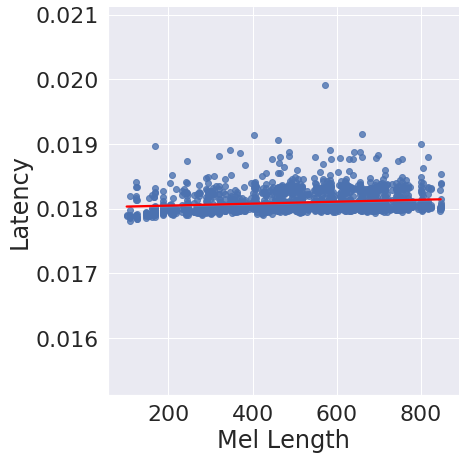
\includegraphics[width=1.0\textwidth]{images/len-lat.png}
\caption{Два шага TTS систем}
\label{fig:len-lat}
\end{figure}